% Options for packages loaded elsewhere
\PassOptionsToPackage{unicode}{hyperref}
\PassOptionsToPackage{hyphens}{url}
%
\documentclass[
]{article}
\usepackage{amsmath,amssymb}
\usepackage{iftex}
\ifPDFTeX
  \usepackage[T1]{fontenc}
  \usepackage[utf8]{inputenc}
  \usepackage{textcomp} % provide euro and other symbols
\else % if luatex or xetex
  \usepackage{unicode-math} % this also loads fontspec
  \defaultfontfeatures{Scale=MatchLowercase}
  \defaultfontfeatures[\rmfamily]{Ligatures=TeX,Scale=1}
\fi
\usepackage{lmodern}
\ifPDFTeX\else
  % xetex/luatex font selection
\fi
% Use upquote if available, for straight quotes in verbatim environments
\IfFileExists{upquote.sty}{\usepackage{upquote}}{}
\IfFileExists{microtype.sty}{% use microtype if available
  \usepackage[]{microtype}
  \UseMicrotypeSet[protrusion]{basicmath} % disable protrusion for tt fonts
}{}
\makeatletter
\@ifundefined{KOMAClassName}{% if non-KOMA class
  \IfFileExists{parskip.sty}{%
    \usepackage{parskip}
  }{% else
    \setlength{\parindent}{0pt}
    \setlength{\parskip}{6pt plus 2pt minus 1pt}}
}{% if KOMA class
  \KOMAoptions{parskip=half}}
\makeatother
\usepackage{xcolor}
\usepackage[margin=1in]{geometry}
\usepackage{graphicx}
\makeatletter
\def\maxwidth{\ifdim\Gin@nat@width>\linewidth\linewidth\else\Gin@nat@width\fi}
\def\maxheight{\ifdim\Gin@nat@height>\textheight\textheight\else\Gin@nat@height\fi}
\makeatother
% Scale images if necessary, so that they will not overflow the page
% margins by default, and it is still possible to overwrite the defaults
% using explicit options in \includegraphics[width, height, ...]{}
\setkeys{Gin}{width=\maxwidth,height=\maxheight,keepaspectratio}
% Set default figure placement to htbp
\makeatletter
\def\fps@figure{htbp}
\makeatother
\setlength{\emergencystretch}{3em} % prevent overfull lines
\providecommand{\tightlist}{%
  \setlength{\itemsep}{0pt}\setlength{\parskip}{0pt}}
\setcounter{secnumdepth}{-\maxdimen} % remove section numbering
\usepackage{titlesec}
\usepackage{xcolor}
\usepackage{ragged2e}
\titleformat{\section}{\color{blue}\Large\bfseries}{\thesection}{1em}{}
\titleformat{\subsection}{\color{blue}\large\bfseries}{\thesubsection}{1em}{}
\titleformat{\subsubsection}{\color{blue}\normalsize\bfseries}{\thesubsubsection}{1em}{}
\titlespacing*{\subsection}{0pt}{*3}{*2}
\titlespacing*{\subsubsection}{0pt}{*3}{*2}
\usepackage{titling}
\pretitle{\begin{center}\LARGE\bfseries\color{blue}}
\posttitle{\par\end{center}\vskip 0.5em}
\preauthor{\begin{center}\large\color{blue}}
\postauthor{\par\end{center}\vskip 0.1em}
\predate{\begin{flushleft}\large\color{blue}}
\postdate{\par\end{flushleft}}
\setlength{\parindent}{0pt}
\setlength{\parskip}{1em}
\renewcommand{\familydefault}{\sfdefault}
\ifLuaTeX
  \usepackage{selnolig}  % disable illegal ligatures
\fi
\usepackage{bookmark}
\IfFileExists{xurl.sty}{\usepackage{xurl}}{} % add URL line breaks if available
\urlstyle{same}
\hypersetup{
  pdftitle={Comprehensive Analysis of U.S. 30-year Climate Normals {[}1991-2020{]}},
  pdfauthor={Anbazhagan Naresh},
  hidelinks,
  pdfcreator={LaTeX via pandoc}}

\title{Comprehensive Analysis of U.S. 30-year Climate Normals
{[}1991-2020{]}}
\author{Anbazhagan Naresh}
\date{June 19, 2024}

\begin{document}
\maketitle

Introduction

\justifying

This document provides a comprehensive analysis of the 30-year climate
normals data for key weather stations in the United States. The dataset,
provided by the National Centers for Environmental Information (NCEI),
includes monthly climate normals for temperature and precipitation for
the period from 1991 to 2020.

Data Acquisition

\justifying

The climate normals data were sourced from the NCEI website. The
inventory and readme files were downloaded to identify key stations and
understand the structure of the dataset. The complete dataset can be
accessed
\href{https://www.ncei.noaa.gov/data/normals-monthly/1991-2020/access/}{\textcolor{blue}{here}}.
The inventory file, which contains a list of all stations and their
metadata, additional documentation explaining the methodology and data
structure is available
\href{https://www.ncei.noaa.gov/data/normals-monthly/1991-2020/doc/}{\textcolor{blue}{here}}.

Key Stations

\justifying

There are over 15000 stations across the United States and for our
convenience of processing this data we identified key stations based on
their Global Surface Network (GSN) and Historical Climatology Network
(HCN) status.The list of key stations is extracted from the provided
inventory file available on the NOAA website.We identified a total of 60
key stations from the inventory file.

Data Cleaning and Aggregation

\justifying

The inventory data were read and cleaned to extract the relevant
information for the key stations. The downloaded CSV files for each
station were then read, and the data were aggregated to compute monthly
averages for temperature and precipitation. Missing values were handled
by removing any incomplete records to ensure data quality.

Data Characteristics

\justifying

This dataframe has 720 rows and 414 columns. The names of the columns
and a brief description of each are in the table below:

Summary Statistics

\justifying

The summary statistics of the cleaned data provide an overview of the
distribution of temperature and precipitation values across the key
stations. The summary includes measures such as the minimum, maximum,
mean, and median values, as well as the first and third quartiles for
each variable. These statistics help us understand the central tendency
and variability in the climate data.

\section*{Visualizations}

Monthly Average Temperature by Station

\justifying

The line plot of monthly average temperature shows the variation in
average temperatures across different stations over the year. This plot
helps identify seasonal trends and compare the temperature profiles of
various stations.

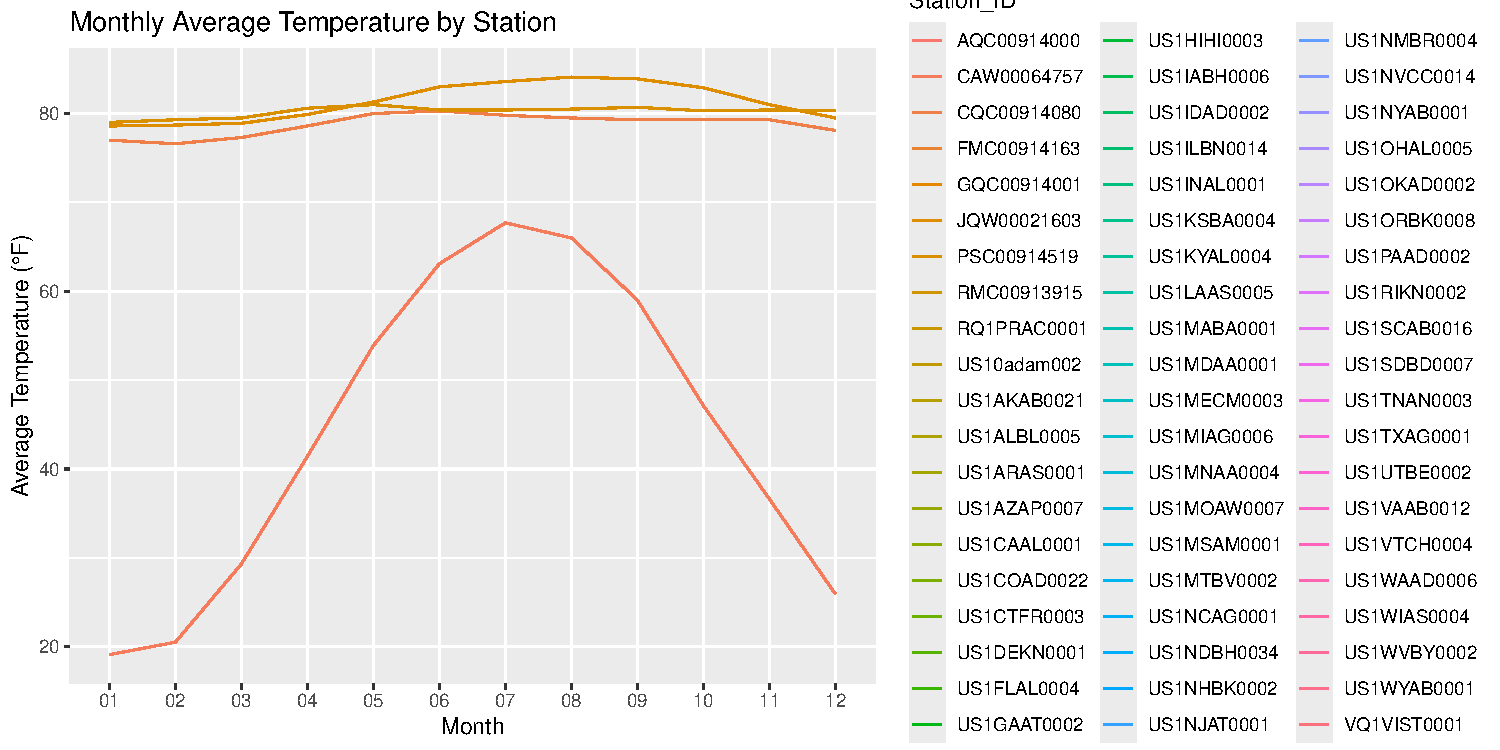
\includegraphics{climate_files/figure-latex/monthly_avg_temp-1.pdf}

Monthly Average Precipitation by Station

\justifying

The line plot of monthly average precipitation illustrates the variation
in precipitation levels across different stations over the year. This
plot helps identify periods of high and low precipitation and compare
precipitation trends among stations.

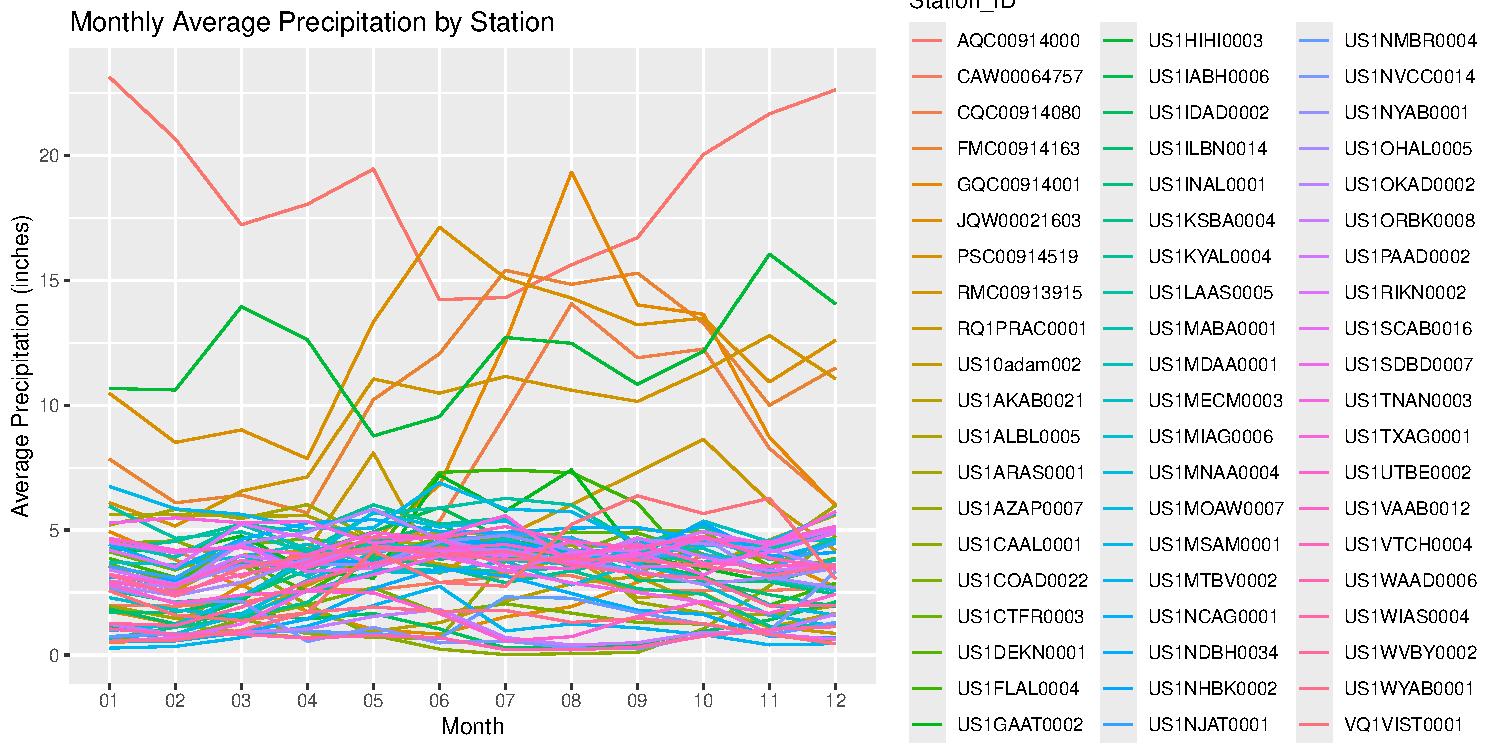
\includegraphics{climate_files/figure-latex/monthly_avg_precip-1.pdf}

Boxplot of Monthly Average Temperature

\justifying

The boxplot of monthly average temperatures reveals several outliers,
represented as individual points beyond the whiskers. These outliers
indicate months where specific weather stations recorded significantly
lower temperatures compared to the overall distribution. For instance,
in January and March, some stations reported average temperatures around
20°F, while in May, June, August, October, November, and December,
outliers around 60°F were observed. These anomalies may be due to
extreme weather events, data collection errors, or unique microclimatic
conditions at specific stations. Further investigation into these
outliers can help validate the data and understand the underlying
climatic factors.

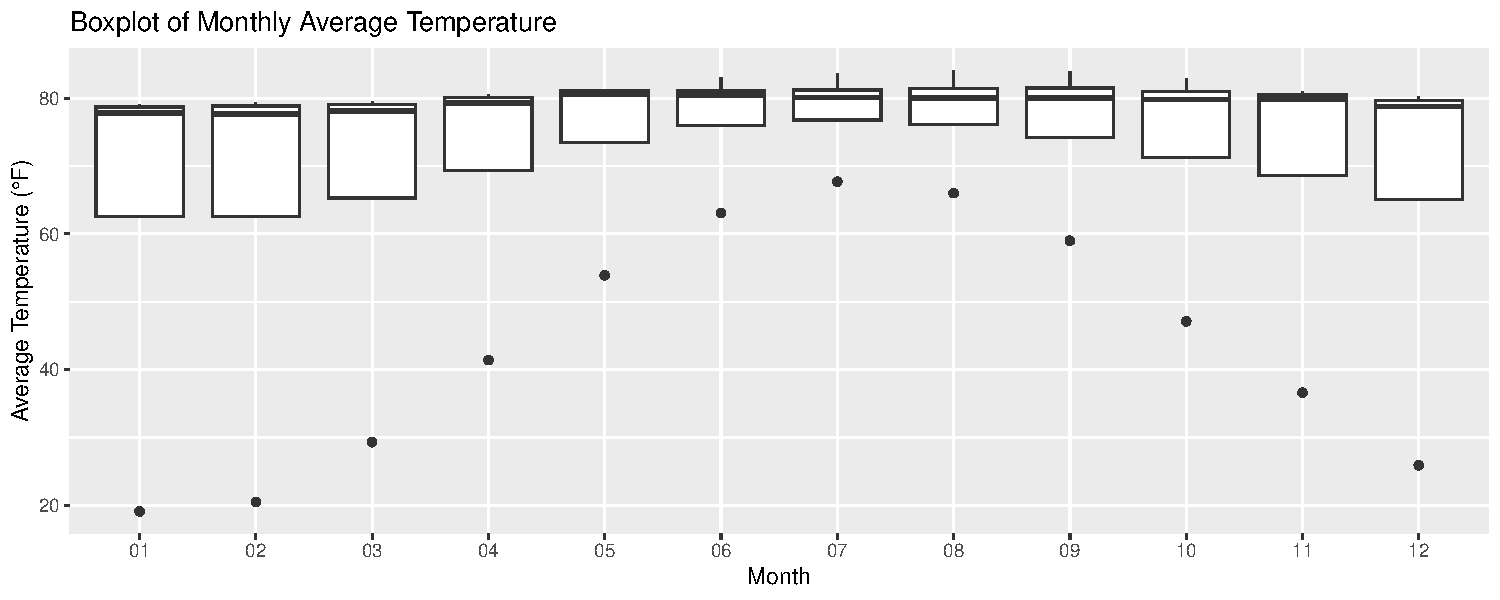
\includegraphics{climate_files/figure-latex/monthly_avg_temp_boxplot-1.pdf}

Boxplot of Monthly Average Precipitation

\justifying

The boxplot of monthly average precipitation shows the distribution of
precipitation levels for each month. Outliers highlight months with
unusually high or low precipitation, which could be due to extreme
weather events or other factors.

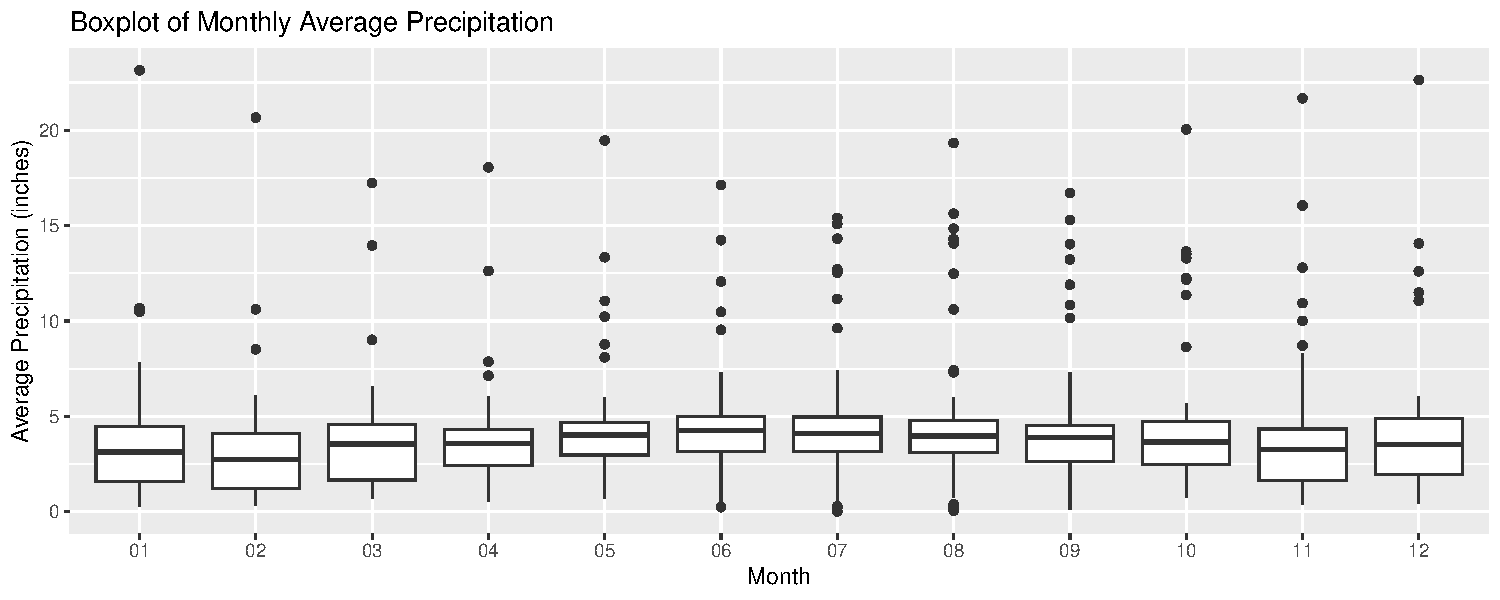
\includegraphics{climate_files/figure-latex/monthly_avg_precip_boxplot-1.pdf}

Heatmap of Monthly Average Temperature

\justifying

The heatmap of monthly average temperature visualizes the temperature
patterns across different stations and months. The color gradient
highlights the variations, with warmer colors indicating higher
temperatures and cooler colors indicating lower temperatures.

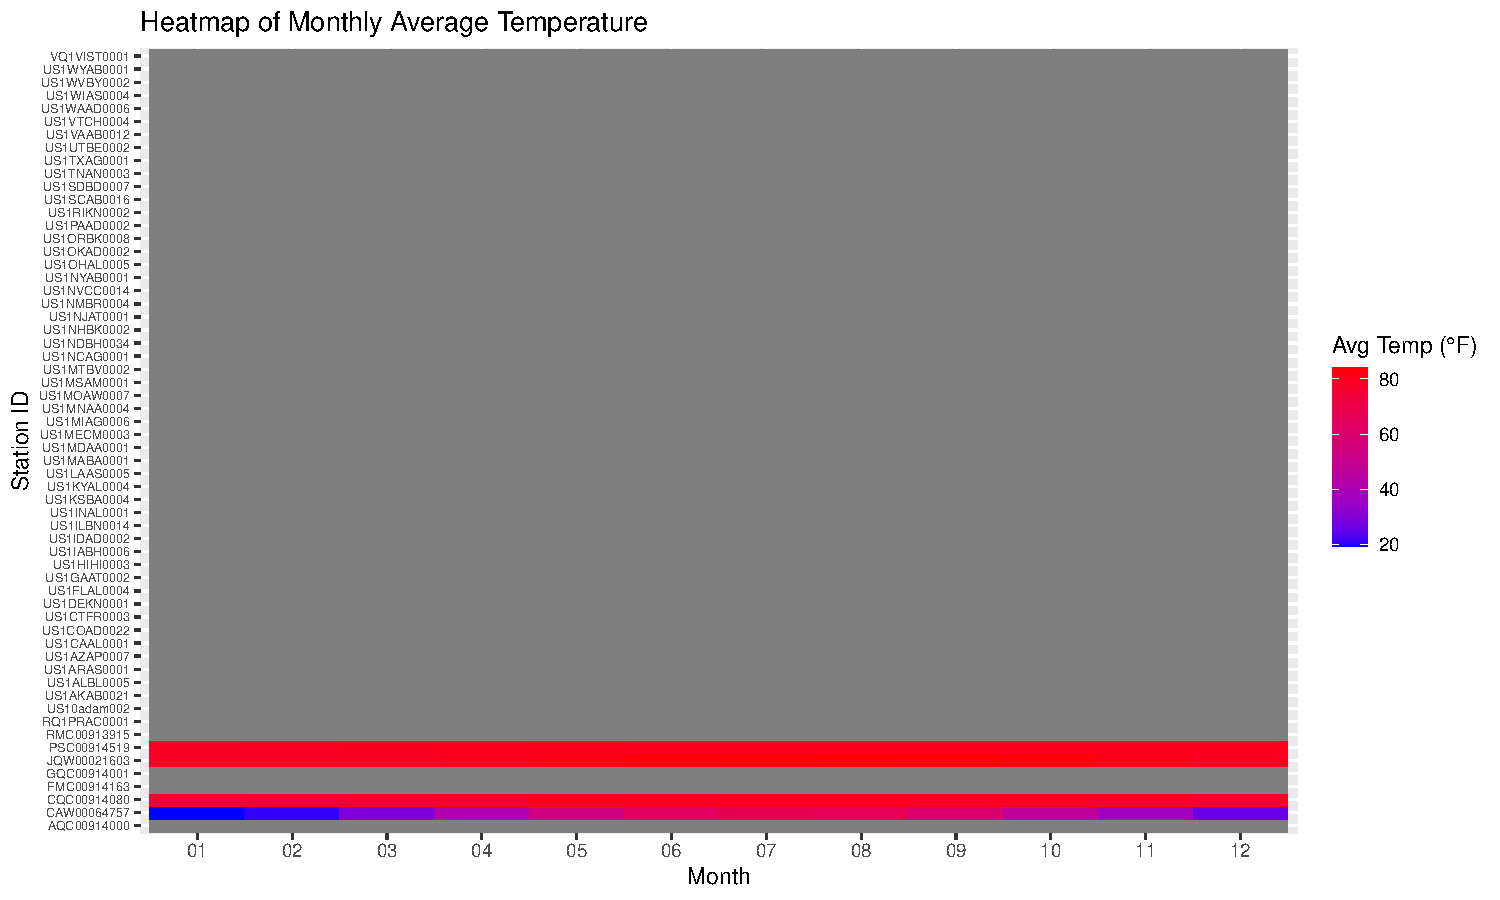
\includegraphics{climate_files/figure-latex/monthly_avg_temp_heatmap-1.pdf}

Heatmap of Monthly Average Precipitation

\justifying

The heatmap of monthly average precipitation displays the precipitation
patterns across different stations and months. The color gradient
highlights the variations, with darker colors indicating higher
precipitation levels.

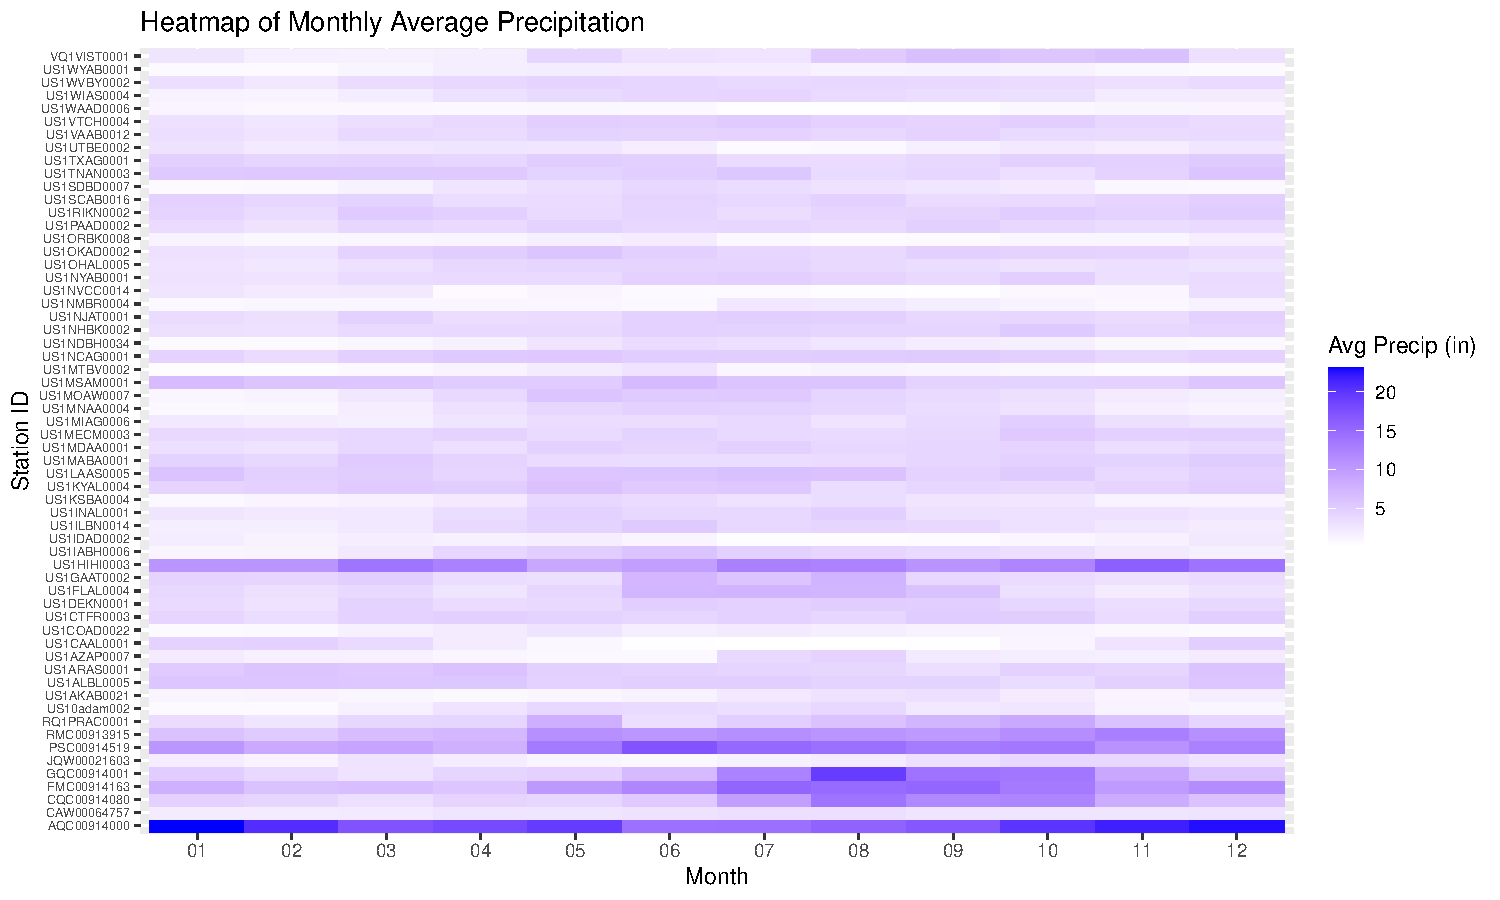
\includegraphics{climate_files/figure-latex/monthly_avg_precip_heatmap-1.pdf}

\justifying

The following maps show the geographical distribution of average
temperature and precipitation for each station. These visualizations
help in understanding the spatial patterns in the climate data.

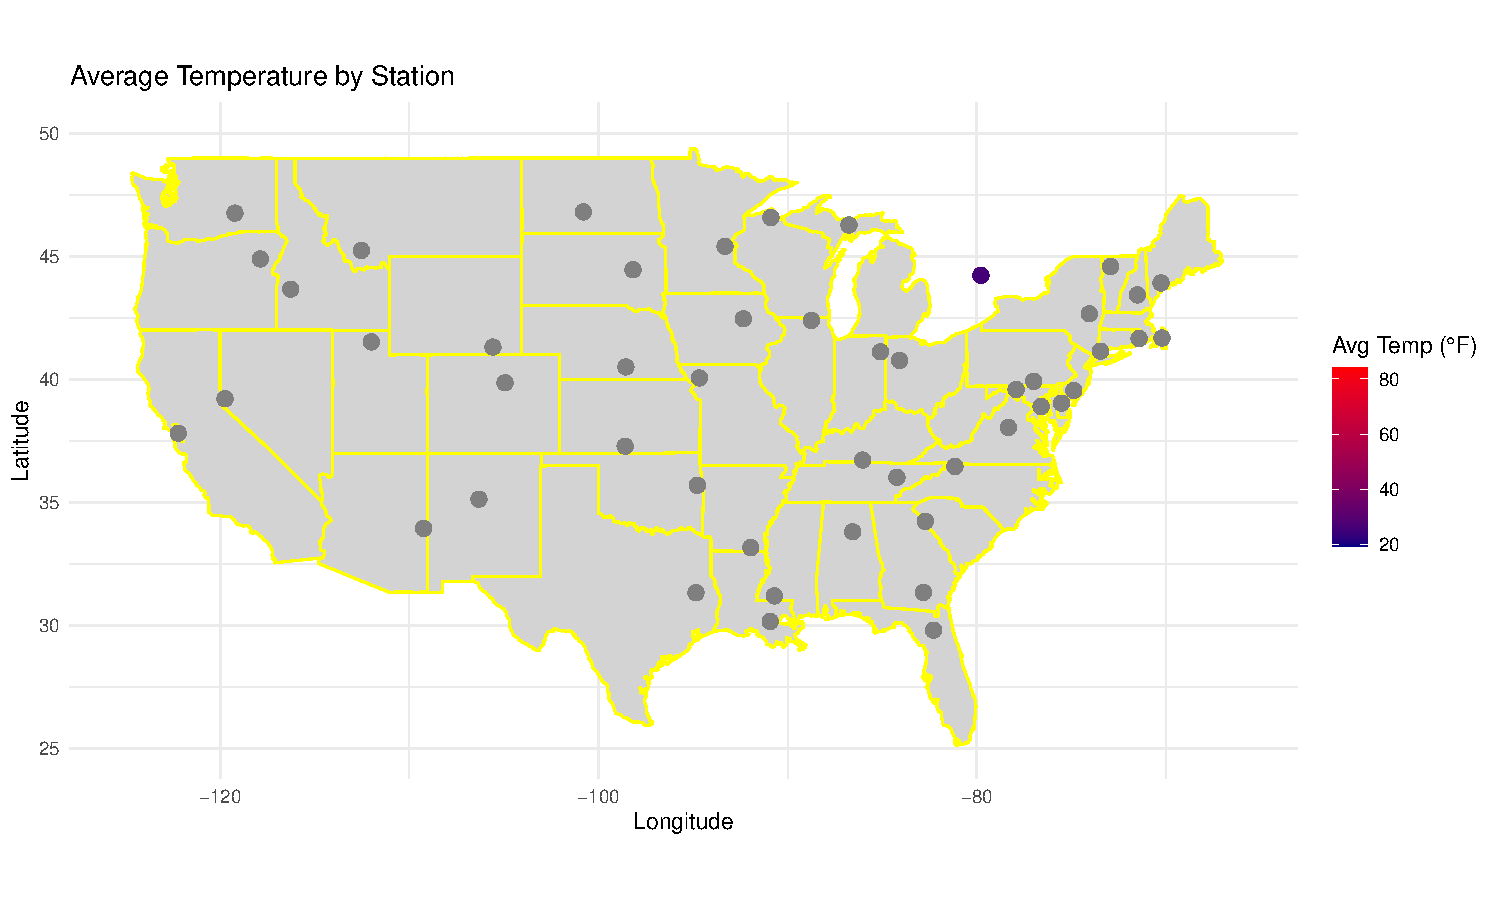
\includegraphics{climate_files/figure-latex/earth_visualization-1.pdf}
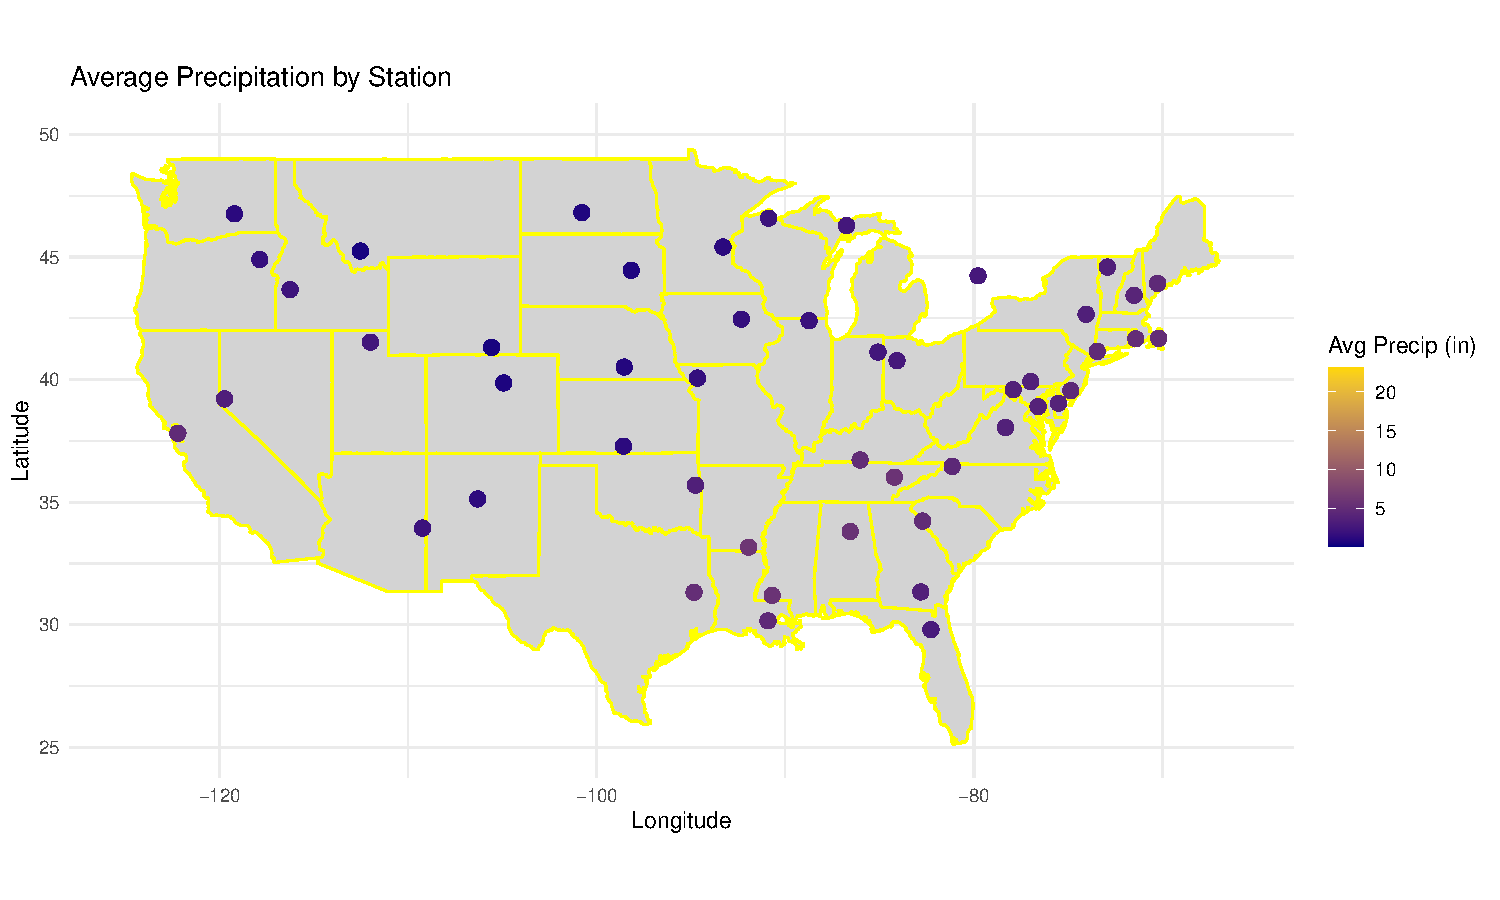
\includegraphics{climate_files/figure-latex/earth_visualization-2.pdf}

\justifying

The following histograms show the distribution of temperatures,
precipitation across all stations to help understand the frequency.

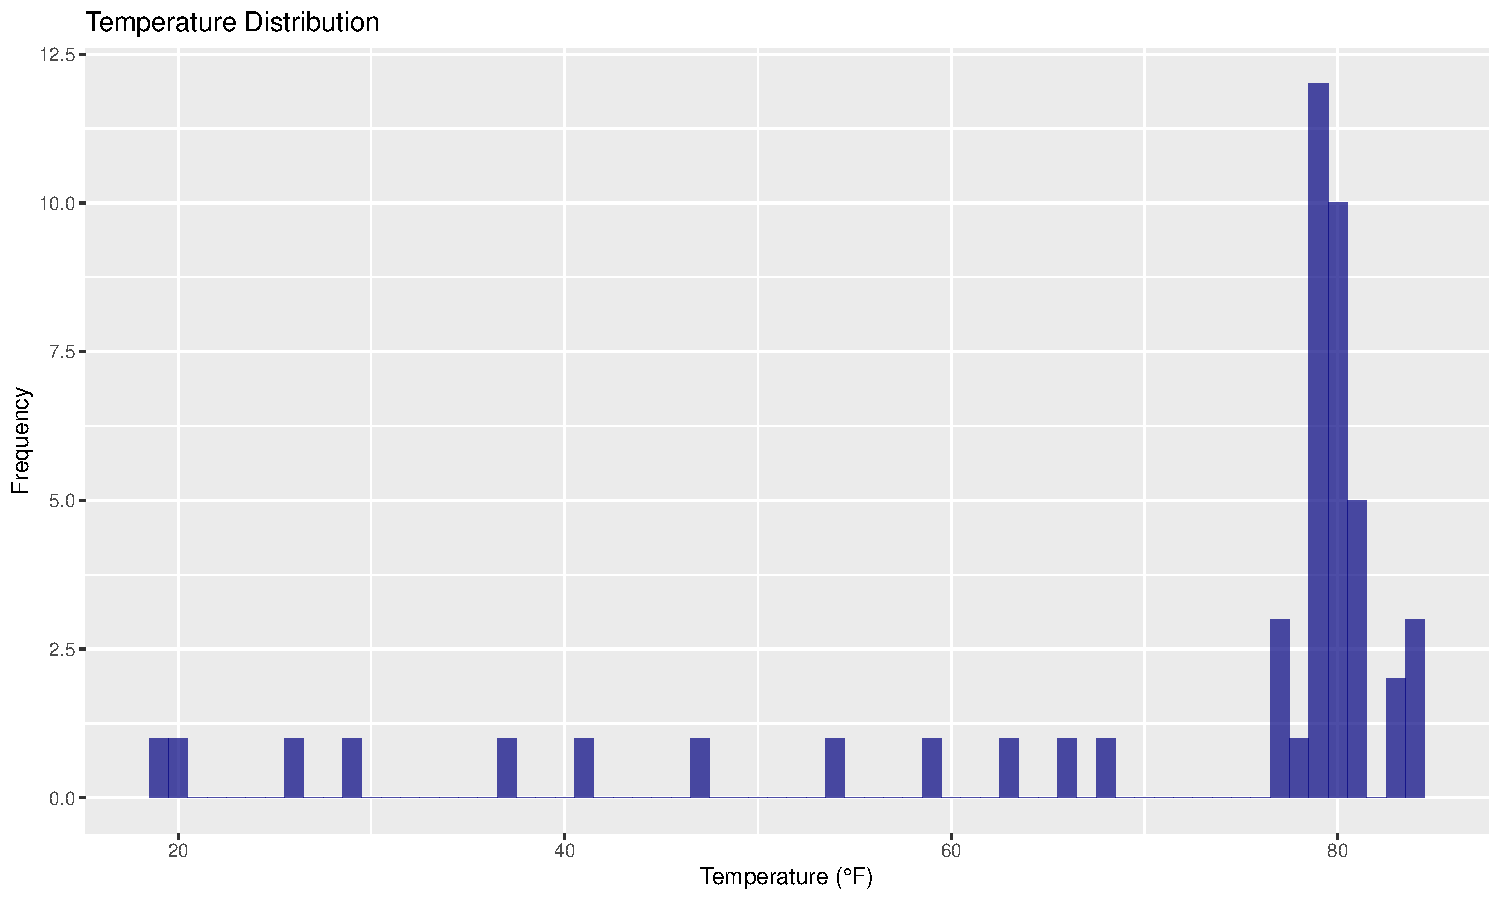
\includegraphics{climate_files/figure-latex/trend_visualization-1.pdf}
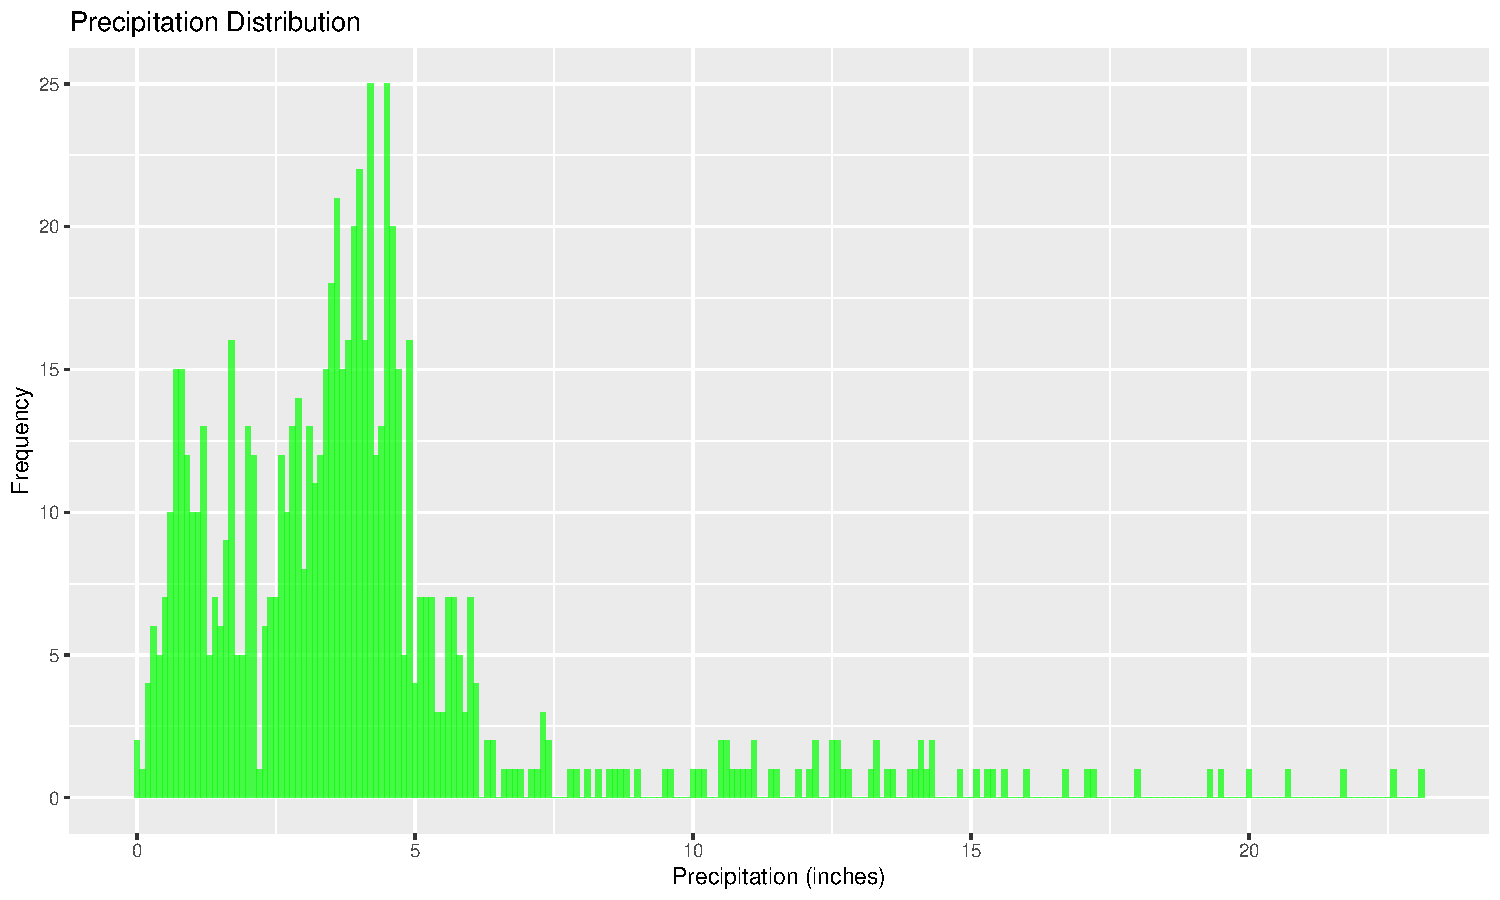
\includegraphics{climate_files/figure-latex/trend_visualization-2.pdf}

\end{document}
